\section{Figures}

\begin{figure}[H]
\centering
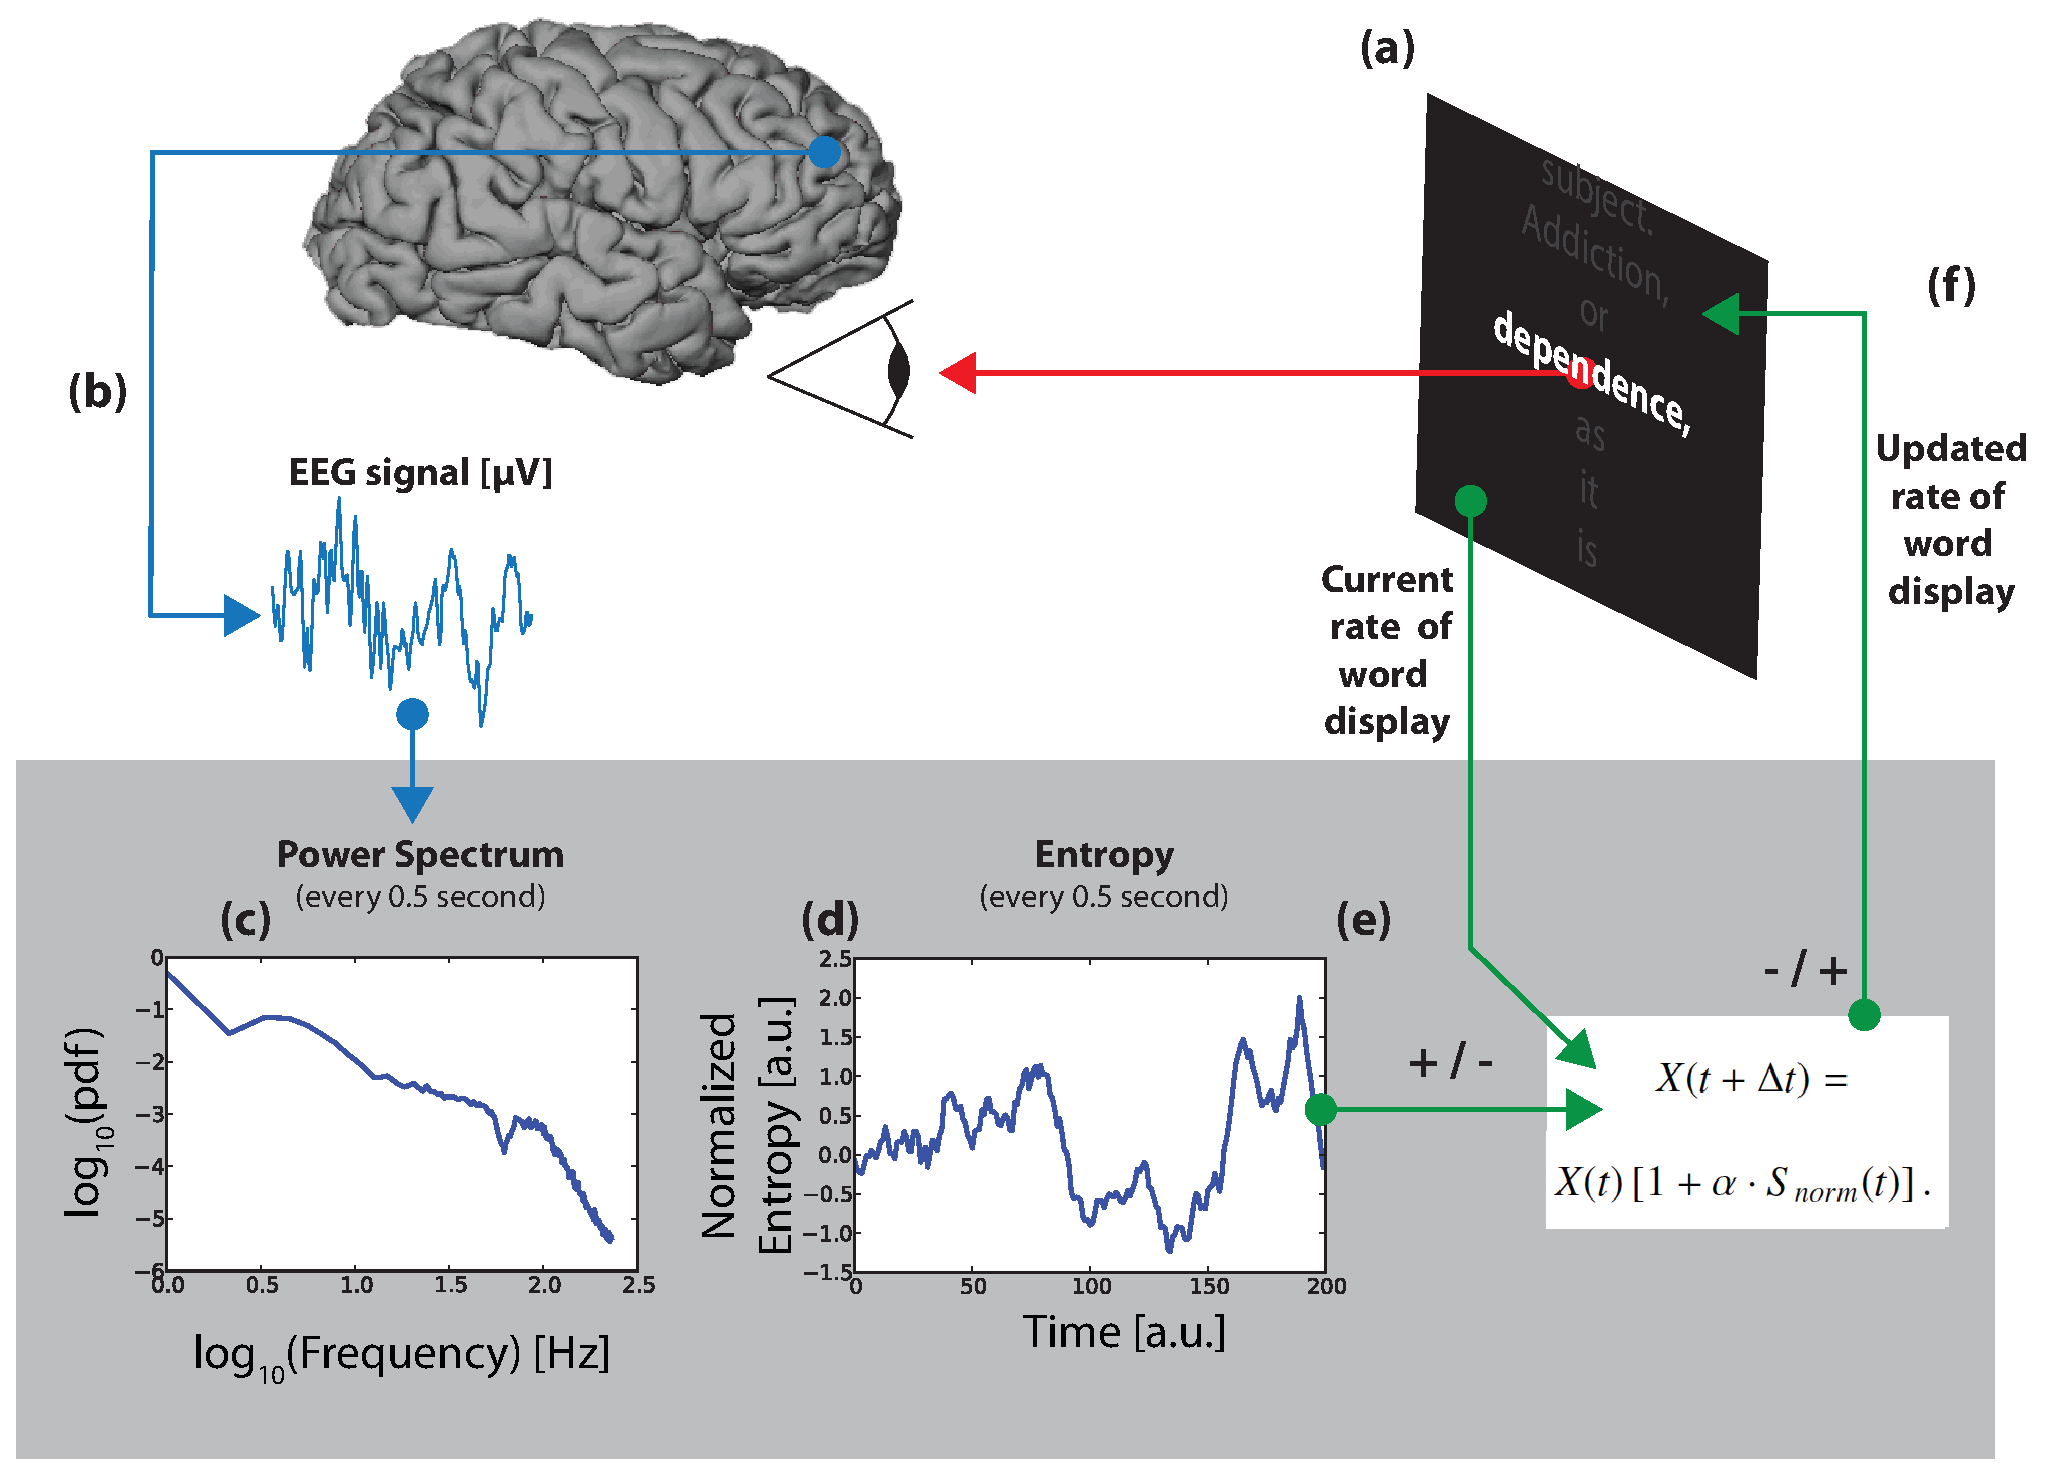
\includegraphics[width=7cm]{../figures2/apparatus.eps}
\caption{Brain speed-reader apparatus: {\bf (a)} Words are displayed and read one after the other at a given rate. {\bf (b)} the EEG signal is recorded through a consumer grade device (here the {\it Neurosky Mindwave}). {\bf (c)} The EEG signal is turned every 0.5 seconds into a power spectrum through a Fourier transform, {\bf (d)} the characteristics of the power spectrum are compressed into a single value characteristic entropy $s$ value. {\bf (e)} A new rate of word display is updated by taking into its current value and $s$. {\bf (f)} The rate of word display is updated accordingly.}
\label{fig:apparatus}
\end{figure}

\begin{figure}[H]
\centering
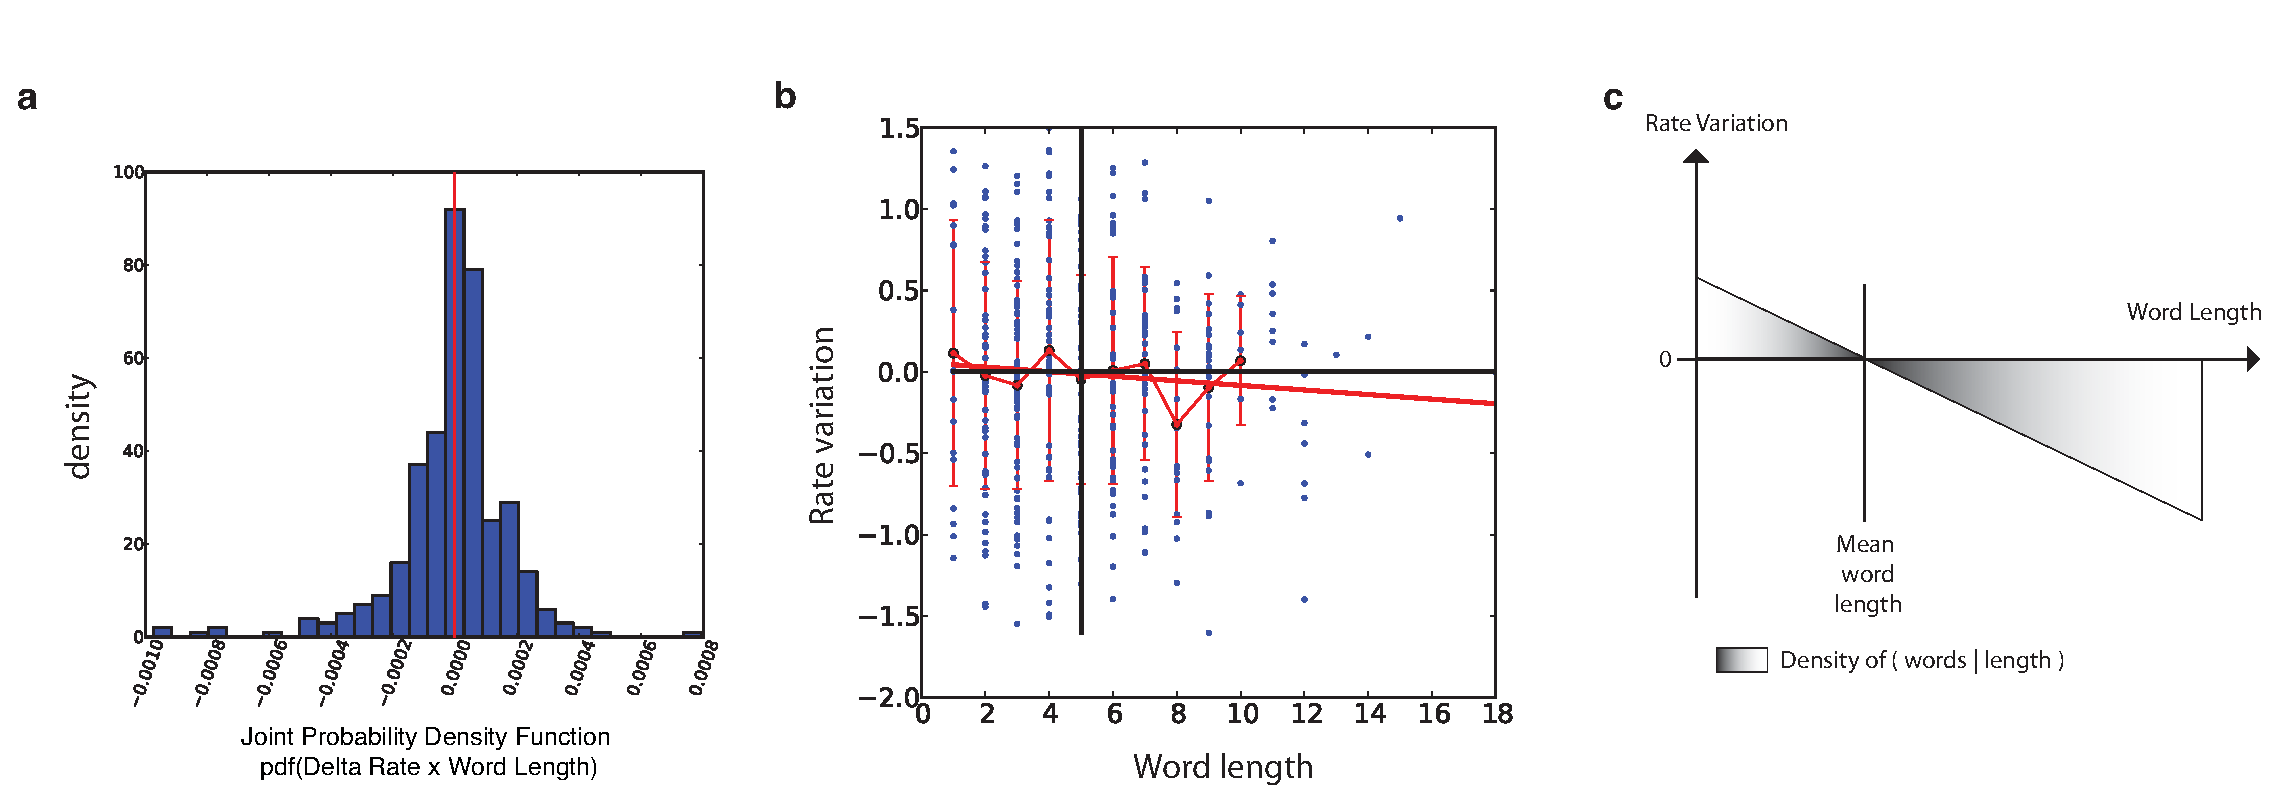
\includegraphics[width=17cm]{../figures2/balance.eps}
\caption{{\bf a.} Schematic representation of the balance of rate change $\Delta_{rate}$ as a function of word length $l_{words}$. The color gradient shows schematically the word density conditioned on their length. This is the canonical or most desirable situation: Around the mean word length the deterministic component of $\Delta_{rate}$ is close to zero. For words with length smaller, the deterministic part of the rate increases, while for words with length larger than the mean, the rate is decreased. The dotted line shows another possible configuration, with acceleration occurring when words are longer. Empirical evidence for the latter case is shown  in Figure \ref{fig:examples} for some typical successful and failed attempts to maintain a balance. ({\bf c}) The joint probability density function $pdf( \Delta_{rate} \times l_{words})$ is well balanced, yet skewed, showing that good control is achieved, along with a good capacity to change the rate of word display.}
\label{fig:apparatus}
\end{figure}

%The linear regression of the average $\Delta_{rates}$ for each word length (for $l_{words} < 10$) exhibits a slope $= 4(1)\times10^{-3}$ ($p < 0.01$). The intersection of $l_{words}(\Delta_{rates} =0) = 4.43$ very close to the average word length (in the text). The error bars show the dispersion (standard deviation of  $\Delta_{rates}$ for each word length. This dispersion is rather large reflecting the stochastic nature of complex brain activation sand the coarse measure obtained from the single electrode EEG headset.

\begin{figure}[H]
\centering
\includegraphics[width=12cm]{../figures2/examples.eps}
\caption{Four examples of successful and failed neuro-feedback control strategies. For each case, three panels are shown (from left to right): (i) Evolution of rate at each displayed word, (ii) rate change as a function of word length at each time step, and (iii)  rate change in the vicinity of large words (9 or more characters, red line), versus words with smaller than 5 characters (blue). The 90\% confidence intervals (light blue area) are obtained by replacement bootstrapping (100 samples of same size as large words are randomly drawn from small words). {\bf a.} Illustration of a very well controlled RSVP, with a sharp and localized drop of word presentation rate around the time large word occurrence. {\bf b.} Opposite strategy with rate increased around large words. {\bf c.} Yet another neuro-feedback strategy with the rate being controlled after the word has occurred. {\bf d.} Failed strategy: Compared to {\bf a}, {\bf b} and {\bf c} the rate change is consistently negative, hence dragging RSVP towards the lower rate limit. Note also in {\bf c} how the rate change as a function of word length (middle panel) is unbalanced around the 0-rate change (horizontal black line) and the mean word length (vertical black line), on the  contrary to {\bf a}, {\bf b} and {\bf c}.}
\label{fig:examples}
\end{figure}


\begin{figure}[H]
\centering
%\includegraphics[width=12cm]{../figures2/examples.eps}
\caption{Here a figure on how the rate is influenced by the power septrum. The idea is to cherry pick moments of high rate change, and look how the power spectrum (and entropy) influences these changes (keep in mind the smoothing, which should reduce the effects of pSpectrum changes on the rate.).}
\label{fig:S_vs_rate}
\end{figure}

\begin{figure}[H]
\centering
%\includegraphics[width=12cm]{../figures2/examples.eps}
\caption{To measure whether there is an effect in the constant rate case, one must first reverse engineer how the rate influences some power spectrum, and how it influences the rate}
\label{fig:constant_rate}
\end{figure}



